\chapter{Technical Analysis} \label{cha: technicalanalysis}
This chapter will present and analyze the technical foundations of the problems described in Chapter \ref{cha:problemanalysis}. It focuses on surveillance equipment, computer vision techniques, person Re-Identification, image Super-Resolution, and related works.   

\section{Surveillance Equipment and Footage}
\label{subsec:Surveillance_equipment_n_footage}

Surveillance cameras are widely used in both public and private settings, and many different factors can influence the overall quality and consistency of recorded footage. Since such recordings can in some cases be the deciding factor when solving crimes, as presented in Section \ref{subsec:Police_Application}, it is important to be aware of the limitations and challenges that can occur, while also having an overall understanding of the technical structure of the systems \cite{arxiv_superres2021}.
 
\subsection{How Cameras Work}
\label{subsubsec:How_cameras_work}
Fundamentally, a camera functions by processing light and converting it into digital data. First, the light passes through a lens, which focuses it onto an image sensor that is made up of millions of photosites (pixels) that can measure the intensity of the light. These measurements are then converted into electrical signals that represent the brightness and color of the different pixels in the image \cite{unc_camera_pipeline}.
There are many underlying elements that happen as well, which can differ in each camera. For example, digital processing like white balance correction, compression and exposure adjustments are used to create the final image or video stream \cite{unc_camera_pipeline}.
An example of this process can be seen in Figure \ref{fig:camera_pipeline}.

\begin{figure}[H]
    \centering
    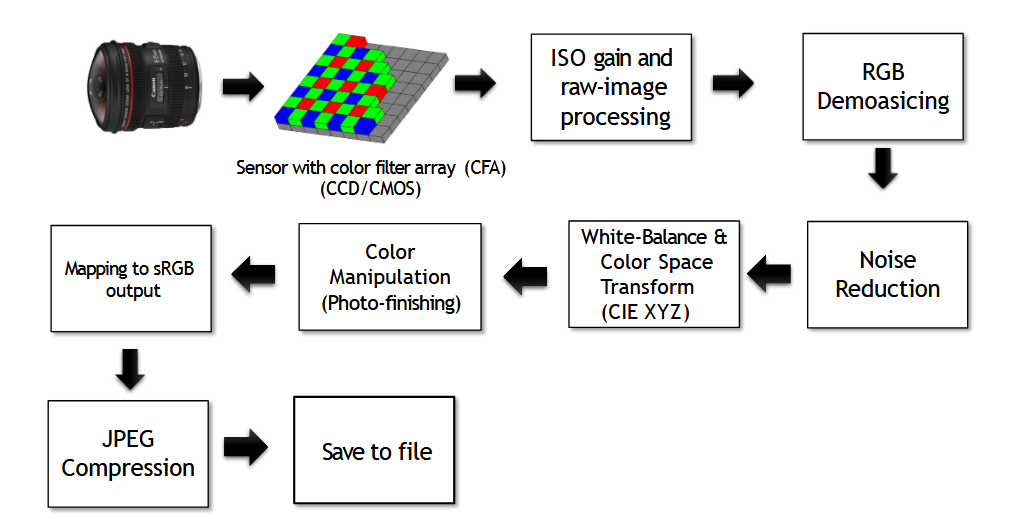
\includegraphics[width=1\linewidth]{figures/images/How_camera_works_pipeline.png}
    \caption{A typical camera pipeline.
    NOTE: This is an example for a standard consumer camera, there are many other cameras which can have different elements in it. }
    \label{fig:camera_pipeline}
\end{figure}
\noindent
These processes mostly differ from camera to camera, which all have their own distinct methods, hardware, settings and quality. This leads to differences in the final footage, an example of this can be seen in Figure \ref{fig:lens_comparison}, where images have different characteristics all depending on the camera used. It is important to understand these fundamental elements when working with surveillance recordings, as they expose the different factors that influence the final output footage, and the way it is processed and worked on \cite{korene_imatest2022_cv_iq}.
\begin{figure}[H]
    \centering
    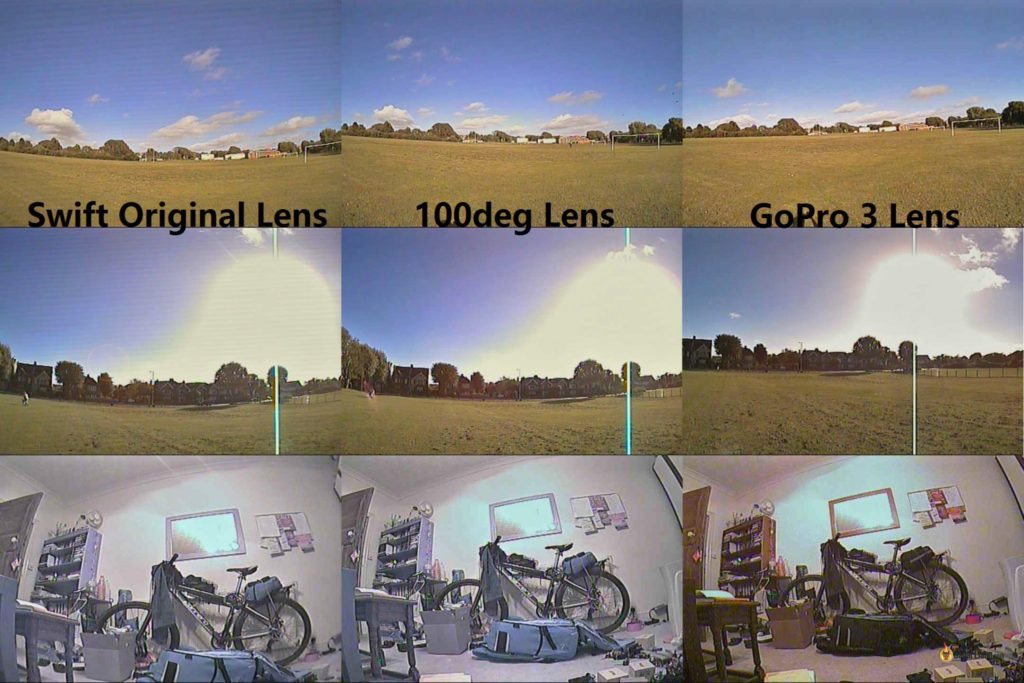
\includegraphics[width=0.7\linewidth]{figures/images/runcam-swift-lens-comparison.jpg}
    \caption{Lens comparison on different cameras to highlight change in color, brightness and \ac{FOV} in the footage.}
    \label{fig:lens_comparison}
\end{figure}
\subsection{Technical Impacts on Footage}
As stated in Section \ref{subsubsec:How_cameras_work}, there are multiple different factors that can influence the overall output of the image. The cameras themselves are rarely alike in terms of quality and features, and some have further restrictions on resolution and refresh rate to reduce energy consumption and storage, while others are able to deliver clearer images with higher resolution and smoother frame rates. In addition, certain cameras include extra functionalities such as night vision, infrared (\acs{IR}), or pan tilt-zoom (\acs{PTZ}) \cite{nightvision_enhancement2018}. This is important to be aware of when working with \ac{AI}, as computer vision works by analyzing and learning the different pixel patterns in images and videos \cite{common_challenges_image_class2024}, which, if not done correctly, can cause unwanted biases for the \acs{AI}-model when used on other surveillance systems by fixating on unimportant noise that would not be present in other instances \cite{opencv2025visionproblems}.

\subsection{Environmental Impacts on Footage}
As surveillance cameras are used for many different tasks, they will be placed in a variety of situations and conditions. Just like how the internal hardware and software can cause challenges when using \acs{AI}, the external factors such as location, season, and weather can create difficulties as well. For example, there are a lot of differences in footage from a camera that is placed inside rather than outside where weather like rain or snow can create noise which reduce clarity and usefulness in the final footage. In contrast, a camera inside is not affected by this, and therefore is viewed differently by the model \cite{arxiv_superres2021}. 
\\\\
Other aspects that can influence the models ability to generalize is light. Many surveillance cameras are used at night, where minimal visibility is achieved with a spotlight or \acf{IR} filters \cite{nightvision_enhancement2018}. However, cameras in well-lit areas have no use for these filters.
\\\\
Footage quality gets worse the greater distance it is recording. As seen in Figure \ref{fig:camera_distance}, subjects further away from the camera get blurrier and more unrecognizable, which is also one of the reasons for implementing a \acs{SR} system, that can create usable data of such cases. 
\begin{figure}[H]
    \centering
    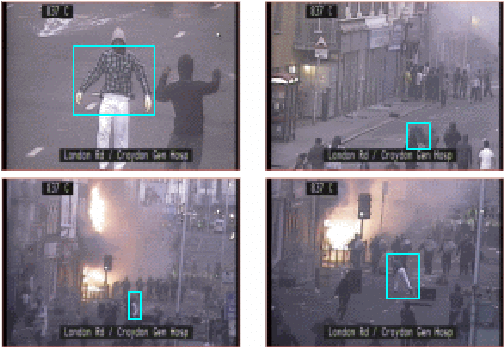
\includegraphics[width=0.7\linewidth]{figures/images/Typical-images-from-a-single-CCTV-camera-with-poor-lighting-and-long-range-camera-views.png}
    \caption{Picture from a surveillance camera in poor light and different distances to the subject marked with a cyan box.}
    \label{fig:camera_distance}
\end{figure}

\section{Computer Vision}
Denne sektion skal danne bro imellem den fysiske/kamera delen af kamera, og hvordan det omdannes til information som en maskine kan bruge. 
\\ ReID afsnittet vil senere uddybe hvordan et ReID netværk forvandler denne information til vektorer (embedding), og derfra kan genkende personer. Danner også grundlaget for at forklare forskellen på billedbaseret ReID og videobas
\\ 

\subsection{Frames as Information}
Hvad information indeholder en billedfil og hvordan indsamles/bruges denne?
\\ Lys, farver, tekstur osv. 

\subsection{Frames in a Time Series}
Hvad yderligere information kan man få fra billeder i en tidsrække? 
\\ Bevægelse, lysændringer, konsistens af objekter osv.

\section{Neural Networks}



\section{Re-identification}


\subsection{Metric Learning}


\subsection{Image-based Re-identification}


\subsection{Video-based Re-identification}


\subsection{Evaluation Metrics}


\subsection{Challenges in Surveillance Re-identification}


\section{Super-Resolution}
\label{sec:SuperResolution}

Surveillance images captured from large distances or in poor lighting conditions often result in low resolution, where important details such as facial features and clothing patterns become unclear. Super-Resolution (SR) is an image processing technique that reconstructs a High-Resolution (HR) image from one or more Low-Resolution (LR) observations, addressing the degraded imagery challenges described in Section 3.1.

The fundamental challenge with SR is that many distinct HR images can produce the same LR measurement under realistic imaging pipelines, making SR an ill-posed inverse problem without a unique solution. Practical SR systems address this by incorporating prior information about natural images to constrain the solution space \cite{Wang2019Survey,Farsiu2004Survey}. Deep learning has revolutionized SR by learning end-to-end mappings from LR to HR directly from data. The Super-Resolution Convolutional Neural Network (SRCNN) demonstrated that a compact Convolutional Neural Network (CNN) trained on bicubic downsampled pairs can outperform hand-crafted pipelines \cite{dong2015imagesuperresolutionusingdeep}.

\subsection{Downsampling vs. Real LR Images}
\label{subsec:DownsamplingVsReal}

Most academic benchmarks generate LR images by artificially downsampling HR images with bicubic interpolation, creating a domain gap between synthetic training data and real-world deployment scenarios \cite{Agustsson2017NTIRE,Timofte2017NTIRE}. Real LR images are shaped by complex degradations including optical factors (lens Modulation Transfer Function (MTF), defocus, motion blur), sensor limitations (Color Filter Array (CFA) patterns and demosaicing), and in-camera processing (tone mapping, JPEG compression). Models trained only on bicubic data often fail when confronted with these real-world degradation patterns \cite{Cai2019RealSR,Wei2020DRealSR}.

Two strategies bridge this gap. First, collecting real paired datasets like RealSR and DRealSR, which capture scenes at different resolutions and demonstrate improved transfer to real images \cite{Cai2019RealSR,Wei2020DRealSR}. Second, synthesizing realistic degradations during training, exemplified by Real-ESRGAN, which applies varying blur kernels, noise models, and compression artifacts to create diverse training data that better mimics real camera pipelines \cite{Wang2021RealESRGAN}.

Evaluation metrics depend on the test data characteristics. Peak Signal-to-Noise Ratio (PSNR) and Structural Similarity Index (SSIM) work well for bicubic benchmarks \cite{Wang2004SSIM}, while Learned Perceptual Image Patch Similarity (LPIPS) and Natural Image Quality Evaluator (NIQE) correlate better with human judgment on real-world data \cite{Zhang2018LPIPS,Mittal2013NIQE}. Best practice reports both distortion measures (PSNR/SSIM) for comparability with existing literature and perceptual assessments (LPIPS/NIQE) for practical applicability \cite{Lugmayr2020NTIRE}.

\subsection{Deep Learning Approaches}

Modern SR architectures extend early CNNs with deeper networks, residual connections, and training objectives beyond pixel-wise losses. Super-Resolution Generative Adversarial Network (SRGAN) introduced adversarial training to SR, combining a generator network with a discriminator that distinguishes real from generated images \cite{Ledig2017SRGAN}. The generator uses 16 residual blocks, while training optimizes both adversarial loss (pushing outputs toward the manifold of natural images) and perceptual loss computed in VGG-19 feature space rather than pixel space.

Enhanced SRGAN (ESRGAN) refined this approach with Residual-in-Residual Dense Blocks (RRDB) that remove batch normalization to avoid artifacts, relativistic adversarial training where the discriminator judges relative rather than absolute realism, and improved perceptual loss formulation \cite{Wang2018ESRGAN}. These refinements enabled significantly sharper textures, winning the Perceptual Image Restoration and Manipulation (PIRM) 2018 perceptual SR track.

Recent real-world variants like Real-ESRGAN incorporate the realistic degradation pipelines discussed above or employ domain adaptation techniques to improve robustness outside controlled bicubic settings \cite{Wang2021RealESRGAN,Cai2019RealSR}.

\subsection{Perception–Distortion Trade-off and Evaluation}

A central design principle for SR is the formal perception–distortion trade-off, which establishes that minimizing distortion metrics (PSNR/SSIM) while maximizing perceptual quality represents contradictory objectives that cannot be jointly optimized \cite{Blau2018PerceptionDistortion}. Methods prioritizing distortion produce smooth outputs that minimize pixel-wise error but appear blurry. Methods prioritizing perceptual quality introduce realistic high-frequency details that satisfy human observers but incur higher distortion scores.

This trade-off directly impacts application design. Forensic analysis requiring high fidelity should prioritize distortion metrics using L1/L2 losses and accept blur to avoid hallucinating details. Visual display applications should prioritize perceptual quality using adversarial and perceptual losses.

For ReID applications, this presents a critical consideration. If SR introduces perceptual improvements through hallucinated details that do not preserve discriminative features the ReID model was trained to recognize, performance may degrade despite improved visual quality. As discussed in Section 3.3.8, ReID models extract features like clothing color and coarse textures. If SR modifies these features in pursuit of perceptual realism, enhanced images may become less suitable for ReID. Comprehensive evaluation reporting both distortion measures and perceptual assessments enables informed method selection \cite{Zhang2018LPIPS,Mittal2013NIQE,Wang2004SSIM}.

\section{Super-Resolution Re-Identification}

\subsection{Trained Together or Separately}

\subsection{}


\section{Related Work - flyttes?}

\subsection{DeepReID: Deep Filter Pairing Neural Network for Person Re-Identification}

This paper proposes a \ac{FPNN} for person \ac{ReID} that automatically learns features optimal for this task directly from image data, instead of relying on hand-crafted ones \cite{FPNN}. The model uses paired filters, one set for each camera view, to learn how a person’s appearance changes across different cameras. This helps the network adapt to variations in lighting, color, angles, viewpoints, and person positions. The model learns to focus on person-specific features and becomes tolerant to imperfect detections and background clutter. 
\\\\
Despite outperforming state-of-the-art methods at the time, this solution has several limitations. The dataset used is relatively small, with 13,164 images of 1,360 different people, which may introduce bias and limit generalization. While the dataset does represent real-life scenarios of obtained data from surveillance cameras, and lighting is mentioned as a key challenge, there is no analysis of image resolution effects or how they could improve the model’s performance. This gap could be explored through integrating \ac{SR} techniques.  

\subsection{Learning a Deep Convolutional Network for Image Super-Resolution}

This paper proposes a method for single image \ac{SR} called \ac{SRCNN} \cite{SRCNN}. The method directly learns an end-to-end mapping between the low- and high-resolution images and jointly optimizes all layers to learn how to reconstruct fine details and textures from data. The mapping is implemented as a deep \ac{CNN} that takes the \ac{LR} image as the input and outputs the \ac{HR} image.
\\\\
Even though this method achieved superior performance to the state-of-the-art methods, it might not be a good idea to apply the \ac{SRCNN} to a \ac{ReID} problem. This is because \ac{SRCNN} does not know that the goal is \ac{ReID} and might distort useful features in the process of enhancing the image. An ideal \ac{SR} model for \ac{ReID} would enhance features useful for recognition, for example the edges around clothes. 	

\subsection{Resolution-invariant Person Re-Identification}

This paper proposes a method for person \ac{ReID} robust to resolution variance by jointly training a \ac{FFSR} module and a \ac{RIFE} by end-to-end \ac{CNN} learning \cite{FFSR}. \ac{FFSR} enhances the person’s image without focusing on the background. \ac{RIFE} extracts features from low- and high-resolution images through two connected streams, allowing the system to compare people’s appearance regardless of image quality. 
\\\\
Although this method is very promising in combining \ac{ReID} with \ac{SR} it does have the limitation of depending on paired low- and high-resolution images, which are unavailable in real-world settings. 
